\documentclass[12pt, twoside]{article}
\usepackage[letterpaper, margin=1in, head=30pt, headsep=0.1in]{geometry}
\usepackage[english]{babel}
\usepackage[utf8]{inputenc}
\usepackage{amsmath}
\usepackage{amsfonts}
\usepackage{amssymb}
\usepackage{tikz}
%\usetikzlibrary{quotes, angles}

\usepackage{graphicx}
\usepackage{enumitem}
\usepackage{multicol}

%\usepackage{pgfplots}
%\pgfplotsset{width=10cm,compat=1.9}
%\usepgfplotslibrary{statistics}
%\usepackage{pgfplotstable}
%\usepackage{tkz-fct}
%\usepackage{venndiagram}

\usepackage{fancyhdr}
\pagestyle{fancy}
\fancyhf{}
\renewcommand{\headrulewidth}{0pt} % disable the underline of the header
\raggedbottom
\newif\ifmeta
\metatrue %print standards and topics tags

\title{Math AI Worksheet Generator and Formative Assessment System}
\author{Chris Huson}
\date{August 2019}

\fancyhead[RE]{\thepage}
\fancyhead[RO]{\thepage \\ Name: \hspace{3cm}}
%\fancyhead[L]{BECA / Dr. Huson / 10th Grade Geometry\\* 7 June 2019}
%
%\begin{document}
%\subsubsection*{13.7 Homework: Cross sections, distance applications}
\fancyhead[L]{BECA / Dr. Huson / Geometry 03-Volume+angle-bisectors\\* pset ID: 43}

\begin{document}

\subsubsection*{3-7DN-Segment-modeling+volume}
\begin{enumerate}
\item Complete the construction of a line perpendicular to line $l$ through the point $P$. 
  \vspace{4cm}
    \begin{center}
    \begin{tikzpicture}[rotate=30]
      \draw [<->, thick] (-2,0)--(8,0)node[below]{$l$}--(9,0);
      \draw [fill] (4,2) circle [radius=0.05] node[right]{$P$};
    \end{tikzpicture}
    \end{center} \vspace{4cm}
  
\item  A shipping crate is $4 \frac{1}{2}$ feet long, 3 feet wide, and $2 \frac{1}{2}$ tall. Find the volume of the crate. Show the calculation.
  \begin{flushright}
    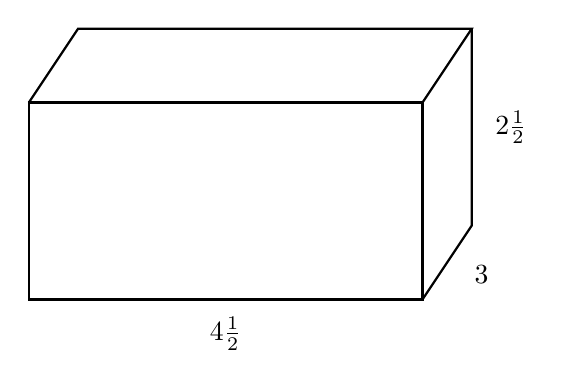
\begin{tikzpicture}[scale=1.25]
      \draw [-, thick] (0,0)--(4,0)--(4,2)--(0,2)--cycle;
      \draw [-, thick] (0,2)--(0.5,2.75)--(4.5,2.75)--(4,2);
      \draw [-, thick] (4,0)--(4.5,0.75)--(4.5,2.75);
      \node at (4.9, 1.75){$2 \frac{1}{2}$};
      \node at (2, -0.35){$4 \frac{1}{2}$};
      \node at (4.6, 0.25){$3$};
    \end{tikzpicture}
    \end{flushright} \vspace{2cm}

    \newpage
    \subsubsection*{Do Not Solve! Complete the drawing on the right and write an equation modeling the situation on the left. Write down a justification, either ``Segment addition postulate'' or ``Definition of a bisector (or midpoint).''}
    \vspace{0.5cm}
  
\item Given $\overline{PQR}$, with $PQ=2x+1$, $QR=5x+3$, and $PR=18$. Find ${PQ}$. \vspace{1cm}
  \begin{flushright}
    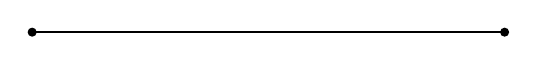
\begin{tikzpicture}
      \draw [-, thick] (0,0)--(6,0);
      \draw [fill] (0,0) circle [radius=0.05];
      \draw [fill] (6,0) circle [radius=0.05];
    \end{tikzpicture}
    \end{flushright} \vspace{2cm}
  
\item Given that $X$ bisects $\overline{MN}$. $MX=x+5$, $MN=30$. Find ${x}$. \vspace{1cm}
  \begin{flushright}
    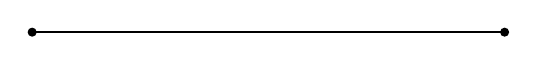
\begin{tikzpicture}
      \draw [-, thick] (0,0)--(6,0);
      \draw [fill] (0,0) circle [radius=0.05];
      \draw [fill] (6,0) circle [radius=0.05];
    \end{tikzpicture}
    \end{flushright} \vspace{2cm}
  
\item The points $A$, $B$, and $C$ are collinear, with $AB=2x+5$ and $BC=22$. If $AC=5x$, find ${AC}$. \vspace{1cm}
  \begin{flushright}
    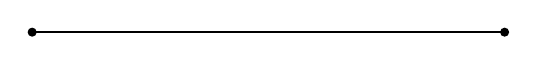
\begin{tikzpicture}
      \draw [-, thick] (0,0)--(6,0);
      \draw [fill] (0,0) circle [radius=0.05];
      \draw [fill] (6,0) circle [radius=0.05];
    \end{tikzpicture}
    \end{flushright} \vspace{2cm}
    
\item The point $E$ is the midpoint of $\overline{DF}$, $DE=3x-5$, and $DF=7x-13$. Find ${DE}$.  \vspace{1cm}
  \begin{flushright}
    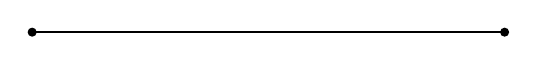
\begin{tikzpicture}
      \draw [-, thick] (0,0)--(6,0);
      \draw [fill] (0,0) circle [radius=0.05];
      \draw [fill] (6,0) circle [radius=0.05];
    \end{tikzpicture}
    \end{flushright} \vspace{2cm}
    
  
\end{enumerate}
\end{document}